\documentclass{beamer}

\usepackage{graphicx}
\usepackage{textpos}
\usepackage{listings}
\usepackage{tikz}
\usepackage{listofitems}

\definecolor{codegreen}{rgb}{0,0.6,0}
\definecolor{codegray}{rgb}{0.5,0.5,0.5}
\definecolor{codepurple}{rgb}{0.58,0,0.82}
\definecolor{backcolour}{rgb}{0.95,0.95,0.92}

\lstdefinestyle{python}{
  backgroundcolor=\color{backcolour},   
  commentstyle=\color{codegreen},
  keywordstyle=\color{magenta},
  numberstyle=\tiny\color{codegray},
  stringstyle=\color{codepurple},
  basicstyle=\ttfamily\footnotesize,
  breakatwhitespace=false,         
  %breaklines=true,                 
  captionpos=b,                    
  keepspaces=true,                 
  %numbers=left,                    
  %numbersep=5pt,                  
  showspaces=false,                
  showstringspaces=false,
  showtabs=false,                  
  tabsize=2
}

\lstset{style=python}

\usetheme{Madrid}
\useoutertheme{miniframes} % Alternatively: miniframes, infolines, split

% Setup the university's color pallette
\definecolor{UIUCorange}{RGB}{19, 41, 75} 
\definecolor{UIUCblue}{RGB}{232, 74, 39} 


\setbeamercolor{palette primary}{bg=UIUCorange,fg=white}
\setbeamercolor{palette secondary}{bg=UIUCblue,fg=white}
\setbeamercolor{palette tertiary}{bg=UIUCblue,fg=white}
\setbeamercolor{palette quaternary}{bg=UIUCblue,fg=white}
\setbeamercolor{structure}{fg=UIUCorange} % itemize, enumerate, etc
\setbeamercolor{section in toc}{fg=UIUCblue} % TOC sections

\setbeamercolor{subsection in head/foot}{bg=UIUCorange,fg=UIUCblue}
\setbeamercolor{subsection in head/foot}{bg=UIUCorange,fg=UIUCblue}

\usepackage[utf8]{inputenc}
\usepackage{graphicx}


%Information to be included in the title page:
\title{\textbf{Introduction to the Course}}
\author{\textbf{David H Smith IV}}
\institute[\textbf{UIUC}]{\textbf{University of Illinois Urbana-Champaign}}
\date{\textbf{Mon, June 14 2021}}

\setbeamertemplate{title page}[default][colsep=-4bp,rounded=true]
\addtobeamertemplate{title page}{\vspace{3\baselineskip}}{}
\addtobeamertemplate{title page}{
  \begin{textblock*}{\paperwidth}(-1.0em, -1.2em)
    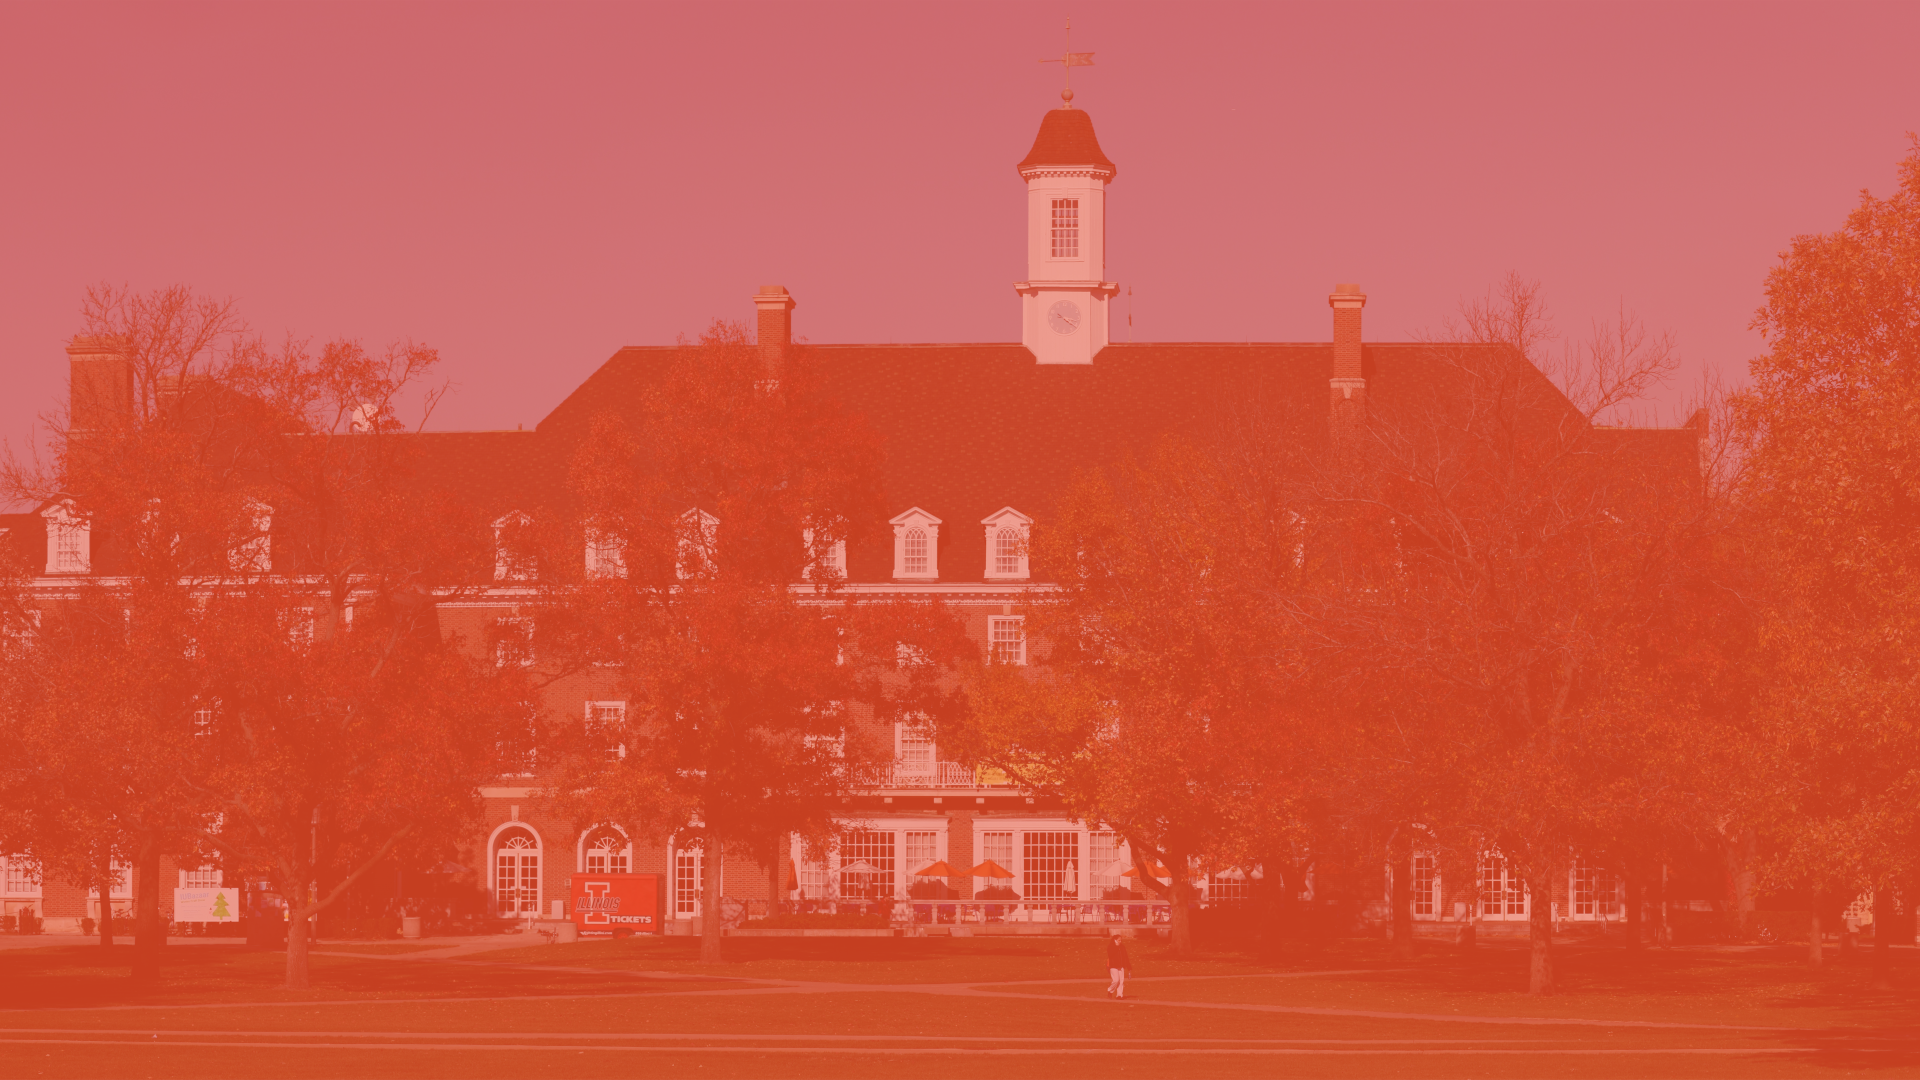
\includegraphics[width=\paperwidth, height=\paperheight]{imgs/uiuc.png}
  \end{textblock*} 
}{}

\begin{document}

\frame{\titlepage}

\section{Course Overview}

%
% Slide 1
%
\begin{frame}
  \frametitle{Course Outcomes}
  \begin{itemize}
    \item Given a small section of code you should be able to:
      \begin{itemize}
        \item Trace through and predict it's output.
        \item Describe, in plain English, what it does.
      \end{itemize}
    \item Write a small python program some using the fundamentals you will learn in this course.
    \item Beginner and intermediate spreadsheet operations.
    \item Beginner level understanding of how the internet works and how to write basic HTML documents.
  \end{itemize}
\end{frame}

\begin{frame}
  \frametitle{Today's Topics}
  \begin{itemize}
    \item Quick overview of the course 
    \item A history of CS and the general purpose computer
    \item The process of constructing programs
  \end{itemize}
\end{frame}

\begin{frame}
  \frametitle{Lecture Time}
  \begin{itemize}
    \item We ask multiple choice questions
    \item You answer the poll individually, for participation points.
    \item Then you discuss with your peers in your assigned lecture discord group.
    \item You will answer the poll a second time for, credit.
  \end{itemize}
\end{frame}

\begin{frame}
  \frametitle{First poll question! - Getting Help}
  \begin{enumerate}
    \item It is okay to hire random internet strangers to do all of your homework for you.
    \item You must do all of your homework alone (not even TAs can help)
    \item You can get any help you want as long as you type in the answers.
    \item Students can only discuss the homework at a high level; code must not be shown to other students, but you can as TAs for help.
    \item Assignments can be done in groups of two students.
  \end{enumerate}
\end{frame}

\section{CS History}

%
% Slide 2
%
\begin{frame}
  \frametitle{What is Computer Science?}
  \begin{itemize}
    \item CS is concerned with understanding:
      \begin{itemize}
        %\pause
      \item Historically concerned with investigating what is computable.
        %\pause
      \item How to compute it in one or more of the following in mind:
        \begin{itemize}
          %\pause
        \item Speed
          %\pause
        \item Reliability
          %\pause
        \item Security 
          %\pause
        \item Resource cost
      \end{itemize}
      %\pause
  \end{itemize}
  \end{itemize}
\end{frame}


%
% Slide 3
%
\begin{frame}
  \frametitle{What is Programming?}
  \begin{minipage}{0.49\textwidth}
    \begin{itemize}
      \item Programming $\neq$ Computer Science
        \begin{itemize}
          \item Rather, programming is a subset of Computer Science
        \end{itemize}
        %\pause
      \item ``Computer Science is no more about computers than astronomy is about telescopes'' - Edsger W. Dijkstra
        %\pause
      \item \textbf{High Level Definition: } A series of instructions that a computer carries out.
    \end{itemize}
  \end{minipage}
  \begin{minipage}{0.49\textwidth}
    \begin{figure}
      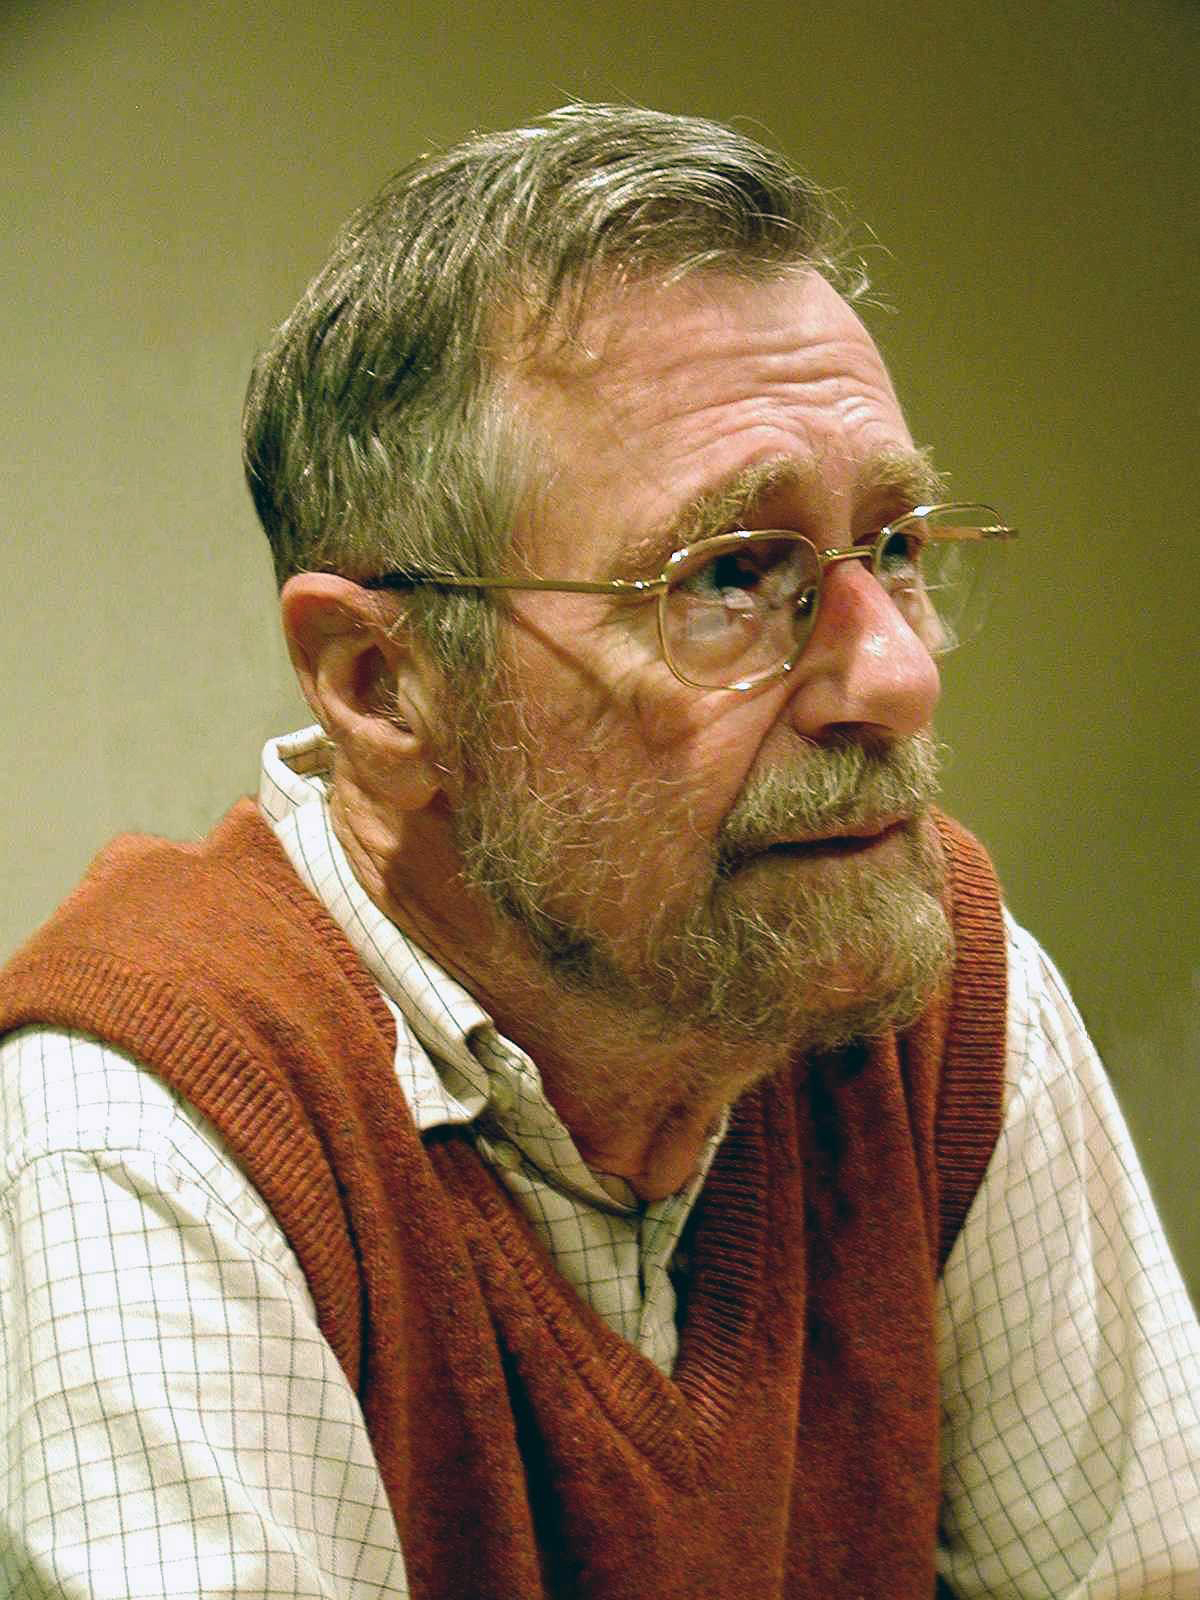
\includegraphics[width=.5\textwidth]{./imgs/dijkstra.jpg}
      \label{fig:dijkstra}
    \end{figure}
  \end{minipage}
\end{frame}

%
%
%
\begin{frame}
  \frametitle{}
  \centering
  \Huge The Journey to a General Purpose Computer
\end{frame}

%
% Slide 5
%
\begin{frame}
  \frametitle{Early ``Computers''}
  \begin{minipage}{0.49\textwidth}
    \begin{figure}
      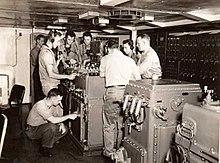
\includegraphics[width=0.5\textwidth]{./imgs/targeting.jpg}
      \label{fig:target}
      \caption{Fire Control System}
    \end{figure}
    \begin{figure}
      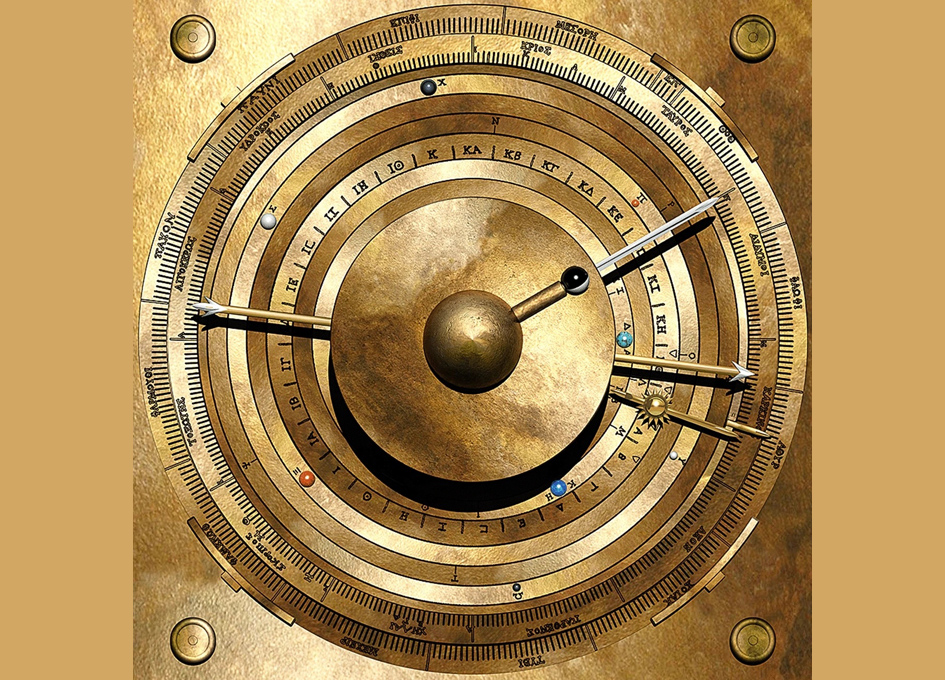
\includegraphics[width=0.5\textwidth]{./imgs/oomechanism.jpg}
      \label{fig:oomechanism}
      \caption{Antikythera Mechanism}
    \end{figure}
  \end{minipage}
  \begin{minipage}{0.49\textwidth}
    \begin{figure}
      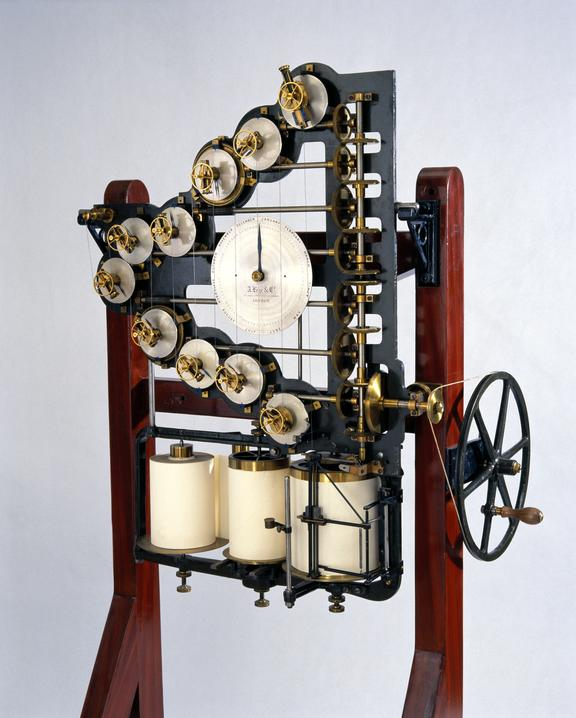
\includegraphics[width=0.5\textwidth]{./imgs/tide.jpg}
      \label{fig:tide}
      \caption{Tide Predicting Machine}
    \end{figure}
  \end{minipage}
\end{frame}

%
% Slide 6
%
\begin{frame}
  \frametitle{The Difference \& Analytical Engines}
  \begin{minipage}{0.59\textwidth}
    \begin{enumerate}
      \item \textbf{Charles Babbage: } Created the Difference Engine and created plans for the Analytical Engine.
      \item \textbf{Ada Lovelace: } The first computer programmer who worked with Babbage on the Analytical Engine.
      \item \textbf{Difference Engine: } A large mechanical calculator capable of performing large computations.
      \item \textbf{Analytical Engine: } The first model of a general purpose mechanical computer.
    \end{enumerate}
    \hfill
  \end{minipage}
  \begin{minipage}{0.39\textwidth}
    \centering
    \begin{figure}
      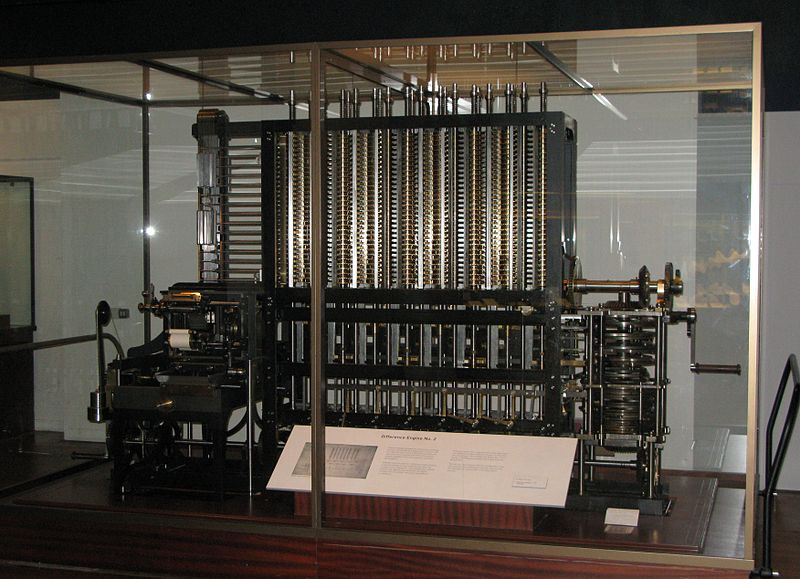
\includegraphics[width=.80\textwidth]{./imgs/differenceengine.jpg}
      \label{fig:analyticalengine.png}
    \end{figure}
    \begin{figure}
      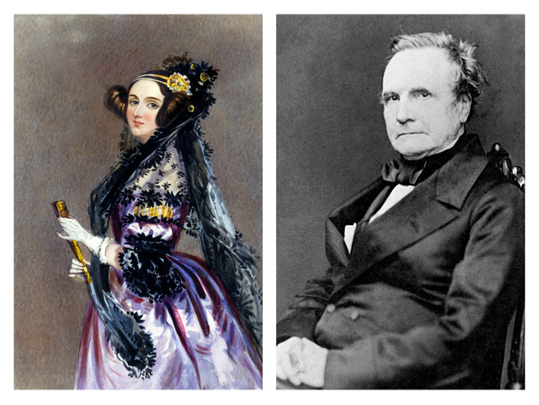
\includegraphics[width=.87\textwidth]{imgs/adababbage.png}
      \label{fig:adababbage.png}
    \end{figure}
  \end{minipage}
\end{frame}

%
% Slide 7
%
\begin{frame}
  \frametitle{Turing Machines}
  \begin{minipage}{0.59\textwidth}
      \textbf{Turing Machines} - An abstract, mathematical model of a machine that moves up and down a strip of paper, one step at a time, and performs operations based on a set of rules.
  \end{minipage}
  \begin{minipage}{0.39\textwidth}
    \begin{figure}
      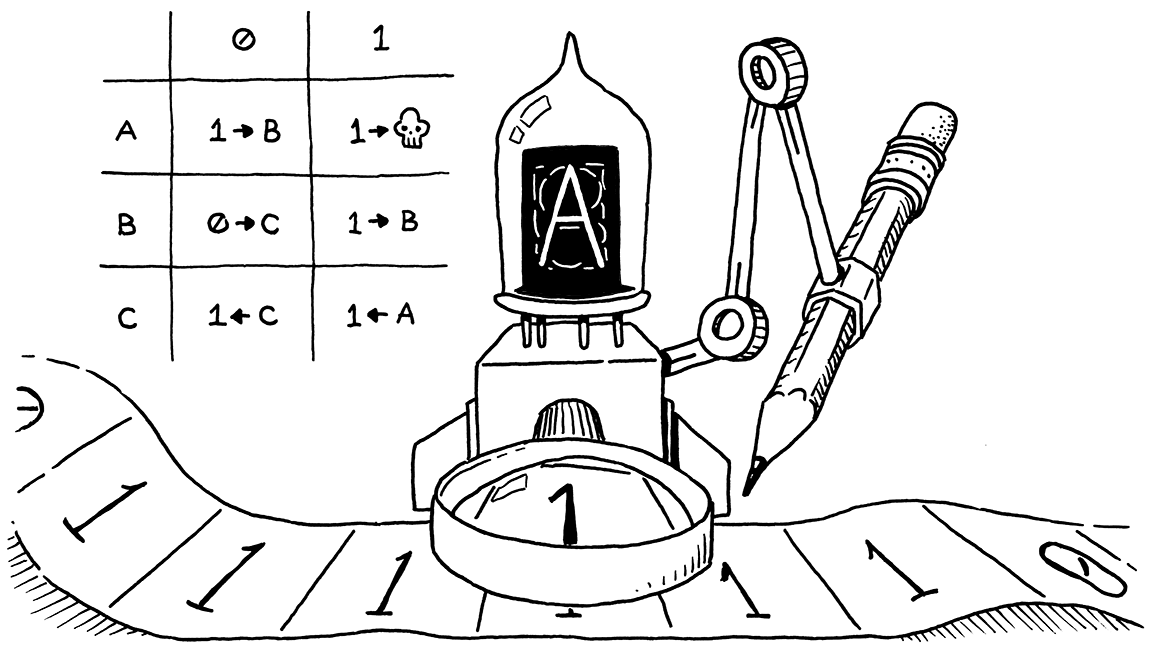
\includegraphics[width=\textwidth]{imgs/turing-machine.png}
      \caption{Artist's Representation of a Turing Machine}
      \label{fig:turingmachine}
    \end{figure}
  \end{minipage}
\end{frame}

%
% Slide 9
%
\begin{frame}
  \frametitle{Von Neumann Architecture}
  \begin{minipage}{0.59\textwidth}
    \begin{enumerate}
      \item \textbf{Input Devices: } Something with buttons and knobs.
        %\pause
      \item \textbf{Central Processing Unit:}
        \begin{enumerate}
          \item \textbf{Control Unit: } Manages everything.
          \item \textbf{Arithmetic/Logic Unit: } Does math and logical comparisons.
        \end{enumerate}
        %\pause
      \item \textbf{Memory Unit: } Supplies info to CPU (i.e., Random Access Memory).
        %\pause
      \item \textbf{External Storage Unit (Not Pictured): } We often need larger storage for data that isn't needed immediately (e.g., Hard Drive).
        %\pause
      \item \textbf{Output Devices: } Flashing lights, monitor, etc.
    \end{enumerate}
  \end{minipage}
  \begin{minipage}{0.39\textwidth}
    \begin{figure}
      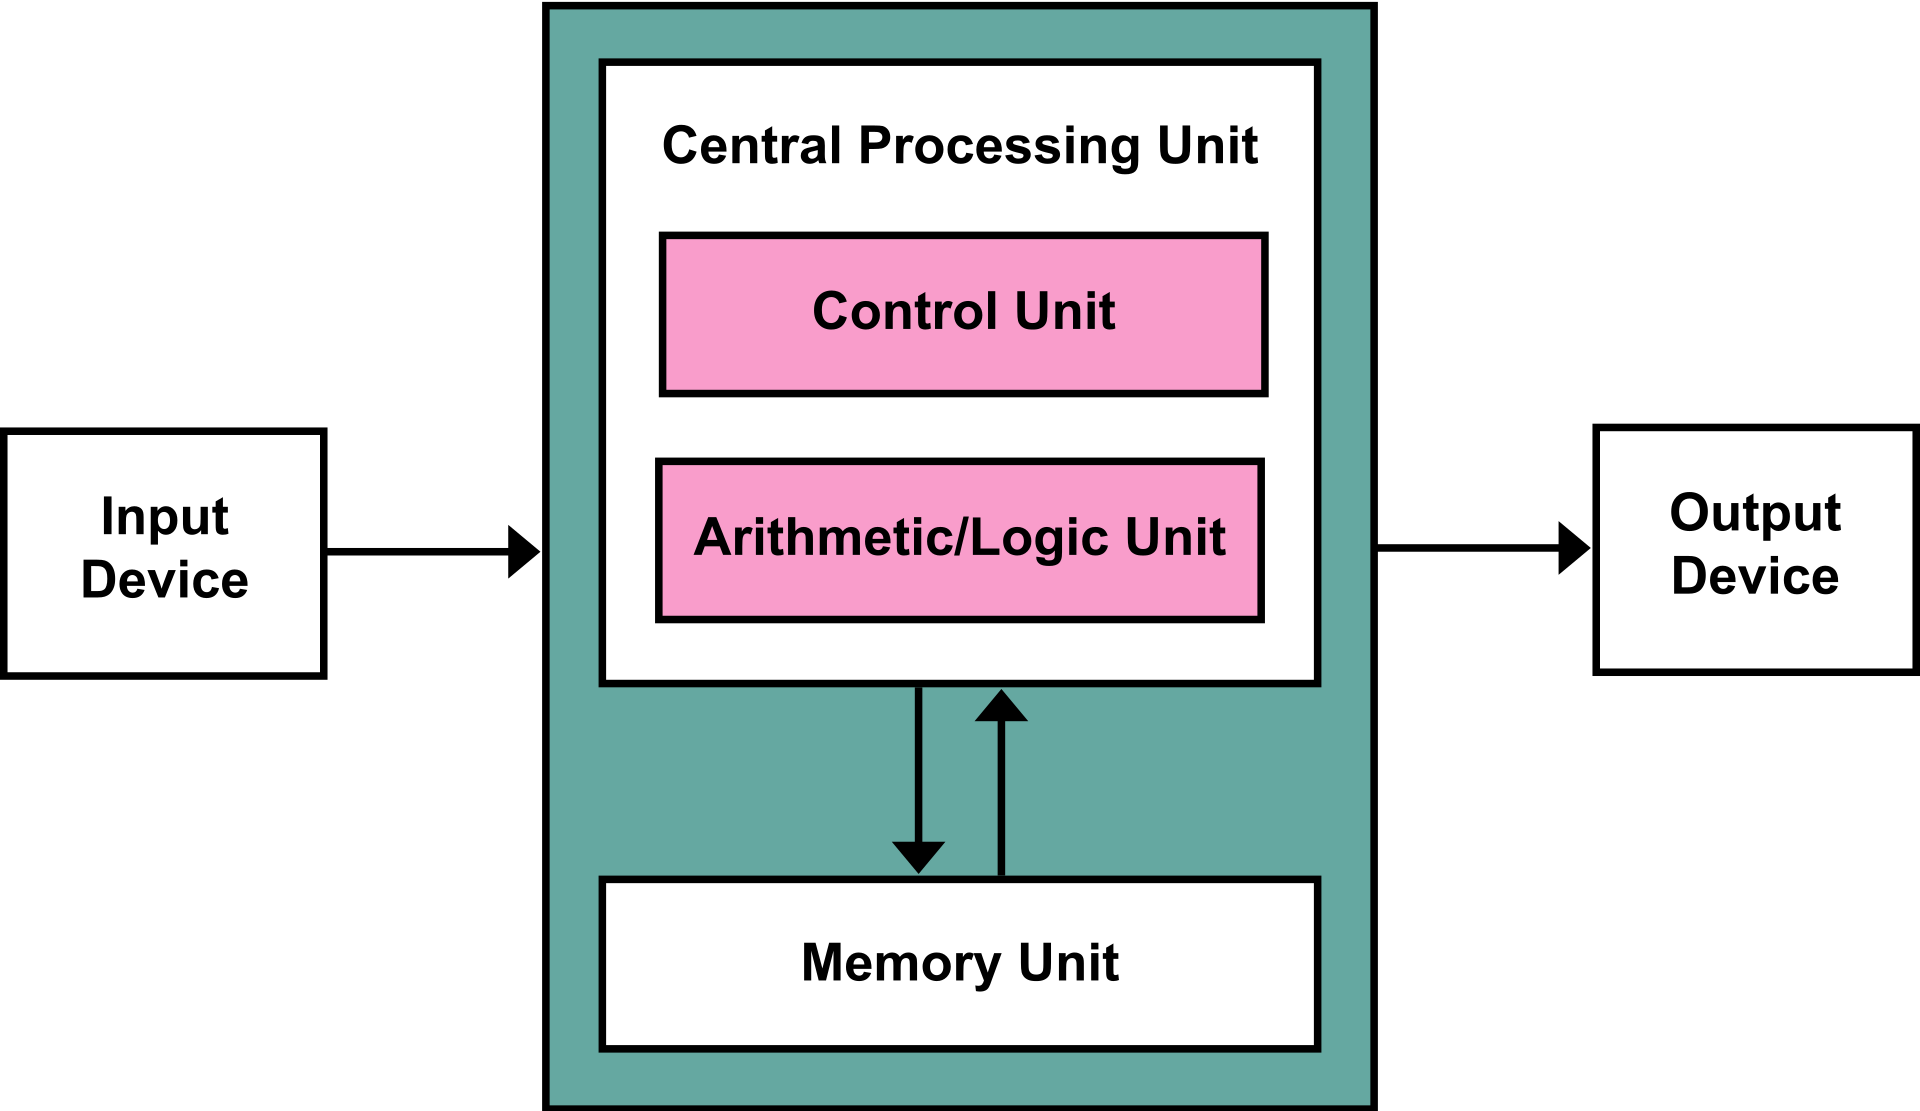
\includegraphics[width=\textwidth]{imgs/von-neumann-arch.png}
      \caption{Von Neumann Architecture}
      \label{fig:vonneumannarch}
    \end{figure}
  \end{minipage}
\end{frame}

%
%
%
\section{How Programs are Constructed}
\begin{frame}
  \frametitle{}
  \centering
  \Huge How Programs are Constructed
\end{frame}

%
% Slide 10
%
%\section{Break}
%\begin{frame}
%  \frametitle{Break time!}
%  \centering
%  \Huge 5 Minute Break
%\end{frame}

%
% Slide
%
\begin{frame}
  \frametitle{Computers Run Low-Level Instructions}
  \begin{minipage}{0.75\textwidth}
    \begin{itemize}
      \item Computers don't ``Play a video''
      \item They\ldots
        \begin{enumerate}
          \item Move some numbers into memory.
          \item Do some math, or a comparison, or both
          \item Make a decision based on the results
          \item Rise a and repeat a few million time before something useful happens
        \end{enumerate}
      \item Programming at this level is:
        \begin{itemize}
          \item Tedious and error prone.
          \item Needs \textbf{\textit{A LOT}} of code to do anything useful.
          \item Isn't portable. Each processor is it's own machine and will require a different set of instructions that works with it's parts.
        \end{itemize}
    \end{itemize}
  \end{minipage}
  \begin{minipage}{0.75\textwidth}
  \end{minipage}
\end{frame}

%
% Slide 10
%
\begin{frame}
  \frametitle{Enter Python (And Other High-Level Languages)}
  \begin{itemize}
    \item They are:
      \begin{itemize}
        \item \textbf{Productive} \textrightarrow A few lines do a lot and it's easy to debug.
          %\pause 
        \item \textbf{Safer} \textrightarrow Less likely to write code that is insecure or damaging.
          %\pause 
        \item \textbf{Portable} \textrightarrow Works on all systems that support the Python interpreter.
      \end{itemize}
    \item Used for everything from machine learning to general scripting.
      %\pause 
    \item We use Python 3.x (not Python 2.x)
  \end{itemize}
\end{frame}

%
% Slide 
%
\begin{frame}
  \frametitle{How programs are Constructed}
  \begin{itemize}
    \item \textbf{Algorithms} \textrightarrow A step-by-step process for achieving a result
      \begin{itemize}
        \item Often Written in pseudo-code
      \end{itemize}
    \item \textbf{Programming} \textrightarrow Express the commands in a form the computer understands.
  \item \textbf{Testing} \textrightarrow Designing inputs that test specific behaviours of the code.
  \item \textbf{Debugging} \textrightarrow Finding errors in the code based on the results of your tests and fixing them.
  \end{itemize}
\end{frame}


%
% Linear Search
%
\section{Algorithms}
%
% Slide
%
\begin{frame}
  \frametitle{A Search Algorithm}
  \begin{minipage}{0.55\textwidth}
    \begin{itemize}
      \item \textbf{Input:} (1) An array of numbers and (2) number for which we're searching.\\
      \item \textbf{Output:} Whether or not the number exists in the list of numbers.\\
      \item \textbf{Algorithm:} \\
      \begin{enumerate}
        \item Look at first item.
        \item Check if it's the item we're looking for.
        \item If it's the item we're looking for stop otherwise go to next item.
        \item Repeat steps 2 \& 3 if there are still items in the list.
      \end{enumerate}
    \end{itemize}
  \end{minipage}
  \hfill
  \begin{minipage}{0.39\textwidth}
    \textbf{Searching Number:} 4\\
    \vspace{0.1cm}\\
    \textbf{Input List:}\\
    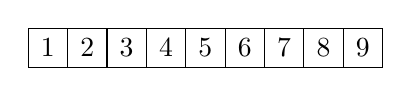
\begin{tikzpicture}
      \draw[draw=black] (0,0) rectangle (.5,.5) node[pos=0.5] {1};
      \draw[draw=black] (.5,0) rectangle (1,.5) node[pos=0.5] {2};
      \draw[draw=black] (1,0) rectangle (1.5,.5) node[pos=0.5] {3};
      \draw[draw=black] (1.5,0) rectangle (2,.5) node[pos=0.5] {4};
      \draw[draw=black] (2,0) rectangle (2.5,.5) node[pos=0.5] {5};
      \draw[draw=black] (2.5,0) rectangle (3,.5) node[pos=0.5] {6};
      \draw[draw=black] (3,0) rectangle (3.5,.5) node[pos=0.5] {7};
      \draw[draw=black] (3.5,0) rectangle (4,.5) node[pos=0.5] {8};
      \draw[draw=black] (4,0) rectangle (4.5,.5) node[pos=0.5] {9};
    \end{tikzpicture}
  \end{minipage}
\end{frame}

\begin{frame}
  \centering
  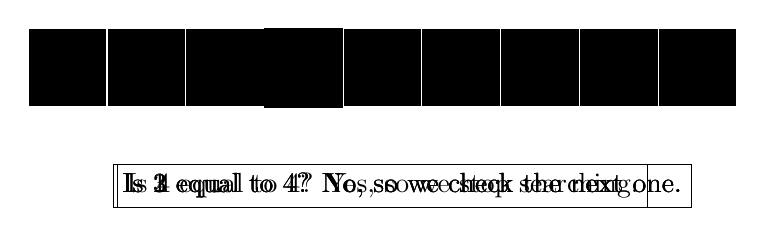
\begin{tikzpicture}
    \pgfmathtruncatemacro{\N}{4}
    \pgfmathtruncatemacro{\asize}{9}
    \foreach \n in {1,2,...,\N}{
      \onslide<\n>{

        \foreach \i in {1,2,3,...,\asize}{
          \ifnum\i=\n
            \draw[draw=black] (\i-1,0) rectangle (\i,1) node[pos=0.5] {\i};
          \else
            \draw[draw=white, fill=black] (\i-1,0) rectangle (\i,1);
          \fi
        }

        \ifnum\n=\N
          \node[draw] at (4.5, -1) {Is \n\ equal to \N? Yes, so we stop searching.};
        \else
          \node[draw] at (4.75, -1) {Is \n\ equal to \N? No, so we check the next one.};
        \fi
      }
    }
  \end{tikzpicture}
\end{frame}



%
% Binary Search
%
%\begin{frame}
  \frametitle{A Search Algorithm}
  \centering
  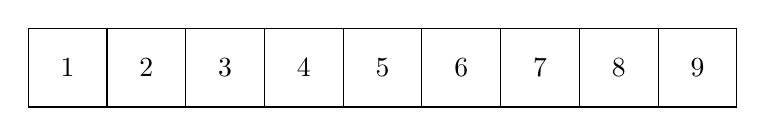
\begin{tikzpicture}
    \draw[draw=black] (0,0) rectangle (1,1) node[pos=0.5] {1};
    \draw[draw=black] (1,0) rectangle (2,1) node[pos=0.5] {2};
    \draw[draw=black] (2,0) rectangle (3,1) node[pos=0.5] {3};
    \draw[draw=black] (3,0) rectangle (4,1) node[pos=0.5] {4};
    \draw[draw=black] (4,0) rectangle (5,1) node[pos=0.5] {5};
    \draw[draw=black] (5,0) rectangle (6,1) node[pos=0.5] {6};
    \draw[draw=black] (6,0) rectangle (7,1) node[pos=0.5] {7};
    \draw[draw=black] (7,0) rectangle (8,1) node[pos=0.5] {8};
    \draw[draw=black] (8,0) rectangle (9,1) node[pos=0.5] {9};
  \end{tikzpicture}
\end{frame}


\begin{frame}
  \frametitle{A Better Search Algorithm}
  \centering
  
\begin{tikzpicture}

    \pgfmathtruncatemacro{\asize}{9}
    \pgfmathtruncatemacro{\N}{3}
    \readlist\values{5,7,8}

    \foreach \n in {1,2,...,\N}{
      \onslide<\n>{
        \foreach \i in {1,2,3,...,\asize}{
          \ifnum\i=\values[\n]
            \draw[draw=black] (\i-1,0) rectangle (\i,1) node[pos=0.5] {\i};
          \else
            \draw[draw=white, fill=black] (\i-1,0) rectangle (\i,1);
          \fi
        }
      }
    }
  \end{tikzpicture}
\end{frame}



%
% Programming
%
\section{Programming}
\begin{frame}[fragile]
  \small 
  \begin{minipage}[t]{0.39\textwidth}
      \textbf{Algorithm:} \\
      \begin{enumerate}
        \item Look at first item.
        \item Check if it's the item we're looking for.
        \item If it's the item we're looking for stop otherwise go to next item.
        \item Repeat steps 2 \& 3 if there are still items in the list.
      \end{enumerate}
  \end{minipage}
  \begin{minipage}[t]{0.59\textwidth}
    \textbf{Code:}
    \begin{lstlisting}[language=Python]
    def search(list, searchitem):
      for item in items:
        if item == searchitem:
          return True
      return False
    \end{lstlisting}
    \hfill
  \end{minipage}
\end{frame}

%
% Slide
%
\begin{frame}
  \frametitle{How Languages are Constructed}
  \begin{itemize}
    \item \textbf{Syntax} \textrightarrow The rules specifying the structure and symbols that are allowable within the programming language.
    \item \textbf{Semantics} \textrightarrow Rules defining the behaviour of symbols or combinations of symbols.
  \end{itemize}
\end{frame}


%
% Slide
%
\begin{frame}
  \frametitle{Testing and Debugging}
  \centering
  \begin{tikzpicture}
    %Sample Inputs
    \draw[draw=black, label=Testing] (0, 0) rectangle (3, 5) node[above, xshift=-1.5cm] {Testing};

    \pgfmathsetseed{\number\pdfrandomseed} 

    \foreach \j in {0, 1, 2, 3, 4}{
      \foreach \i in {0.55, 0.8, 1.05, ..., 2.55}{
        \pgfmathtruncatemacro{\randint}{int(random(0,9))}
        \draw[draw=black] (\i - 0.25, \j + 0.35) rectangle (\i, \j + .6) node[font=\tiny, pos=0.5] {\randint};
      }
      \pgfmathtruncatemacro{\randint}{int(random(5,12))}
      \node[font=\tiny] at (2.75, \j + .475) {\randint};
    }


    \draw[draw=black] (4, 3) rectangle (7, 2) node[pos=.5] {\small Algorithm/Program};

    \draw[draw=black] (8,0) rectangle (11, 5) node[above, xshift=-1.5cm] {Debugging } 
      node[pos=.6, font=\tiny, xshift=-.5cm] {(1) Observe output}
      node[pos=.5, font=\tiny, xshift=-.15cm] {(2) Determine errors}
      node[pos=.4, font=\tiny] {(3) Propose fixes};
    \node[] at (10.75, 5.3) {
\includegraphics[width=.05\textwidth]{imgs/rubberduck.png}};

    \draw[draw=black, ->] (3, 4) -- (4, 3) node[above, pos=.5] {1};
    \draw[draw=black, ->] (7, 3) -- (8, 4) node[above, pos=.5] {2};
    \draw[draw=black, <-] (7, 2) -- (8, 1) node[below, pos=.5] {3};
    \draw[draw=black, <-] (3, 1) -- (4, 2) node[below, pos=.5] {4};

  \end{tikzpicture}
\end{frame}



%
% Slide 
%
\section{Upcoming Material}
\begin{frame}
  \frametitle{Next Lecture Input and Print}
  \begin{itemize}
    \item \underline{\textbf{The Input Function}}: A builtin function that gets a string from the user.
      %\pause
      \begin{itemize}
        \item \textbf{input()} \textrightarrow Doesn't give a prompt.
      %\pause
        \item \textbf{input(``A test input: '')} \textrightarrow Will output the message \textit{"A test input:"} to the screen and let the user type their input in after it.
      %\pause
      \end{itemize}
    \item \underline{\textbf{The Print Function}}: A builtin function that takes a string as a parameter (in between the parentheses) and outputs that string
      %\pause
      \begin{itemize}
        \item \textbf{print(``Hello, World!'')} \textrightarrow Will output the ``Hello, World!''. 
      \end{itemize}
  \end{itemize}
\end{frame}

%
% Slide 
%
\begin{frame}
  \frametitle{Next Lecture: Data Types in Python}
  \begin{itemize}
    \item Two types we'll need to know now:
      \begin{itemize}
        \item \textbf{Strings: } A long list of characters accompanied by surrounding quotes (e.g., ``Hello, CS 105!'').
        \item \textbf{Integers: } Whole numbers, both positive and negative.
      \end{itemize}
    \item You can check the type of a variable or expression with the \lstinline{type()} function.
    %\pause
    \item You can convert between them with the \lstinline{str()} and \lstinline{int()} functions.
    %\pause
    \item It's important to keep the type of your variables in mind when programming.
    %\pause
    \item Keeping types in mind when attempting to deduce what a program is doing is very important. 
  \end{itemize}
\end{frame}



\end{document}
